\chapter{Scientific Background and Terminology}

\section{Polygonal Meshes}

Polygonal meshes are discrete representations of 2D manifold embedded in 3D euclidean space. They and are ubiquitous and fundamental for wide variety of applications such as computer graphics, architecture, virtual and augmented reality, medical imaging, mechanical engineering, computer aided design, geometric deep learning, and much more. Polygonal meshes are composed of the following \emph{elements}:

\begin{itemize}
    \item \emph{Vertices}, points in space.
    \item \emph{Edges}, line-segments that connect two vertices.
    \item \emph{Facets}, polygons made by cycles of edges.
\end{itemize}

\noindent An element might be adjacent to another element. For example, an edge is adjacent to the two vertices which constitutes it; an edge is also adjacent to all faces of which it is part of, and so on. The most common type of polygonal meshes are:

\begin{itemize}
    \item \emph{Triangle mesh}, of which all its facets are triangles.
    \item \emph{Quad mesh}, of which all its facets are quadrilaterals.
    \item \emph{Quad dominant mesh}, of which the majority of facets are quadrilaterals, while there might be additional non-quadrilateral facets, such as triangles and pentagons.
\end{itemize}

\begin{figure}[ht]
\centering
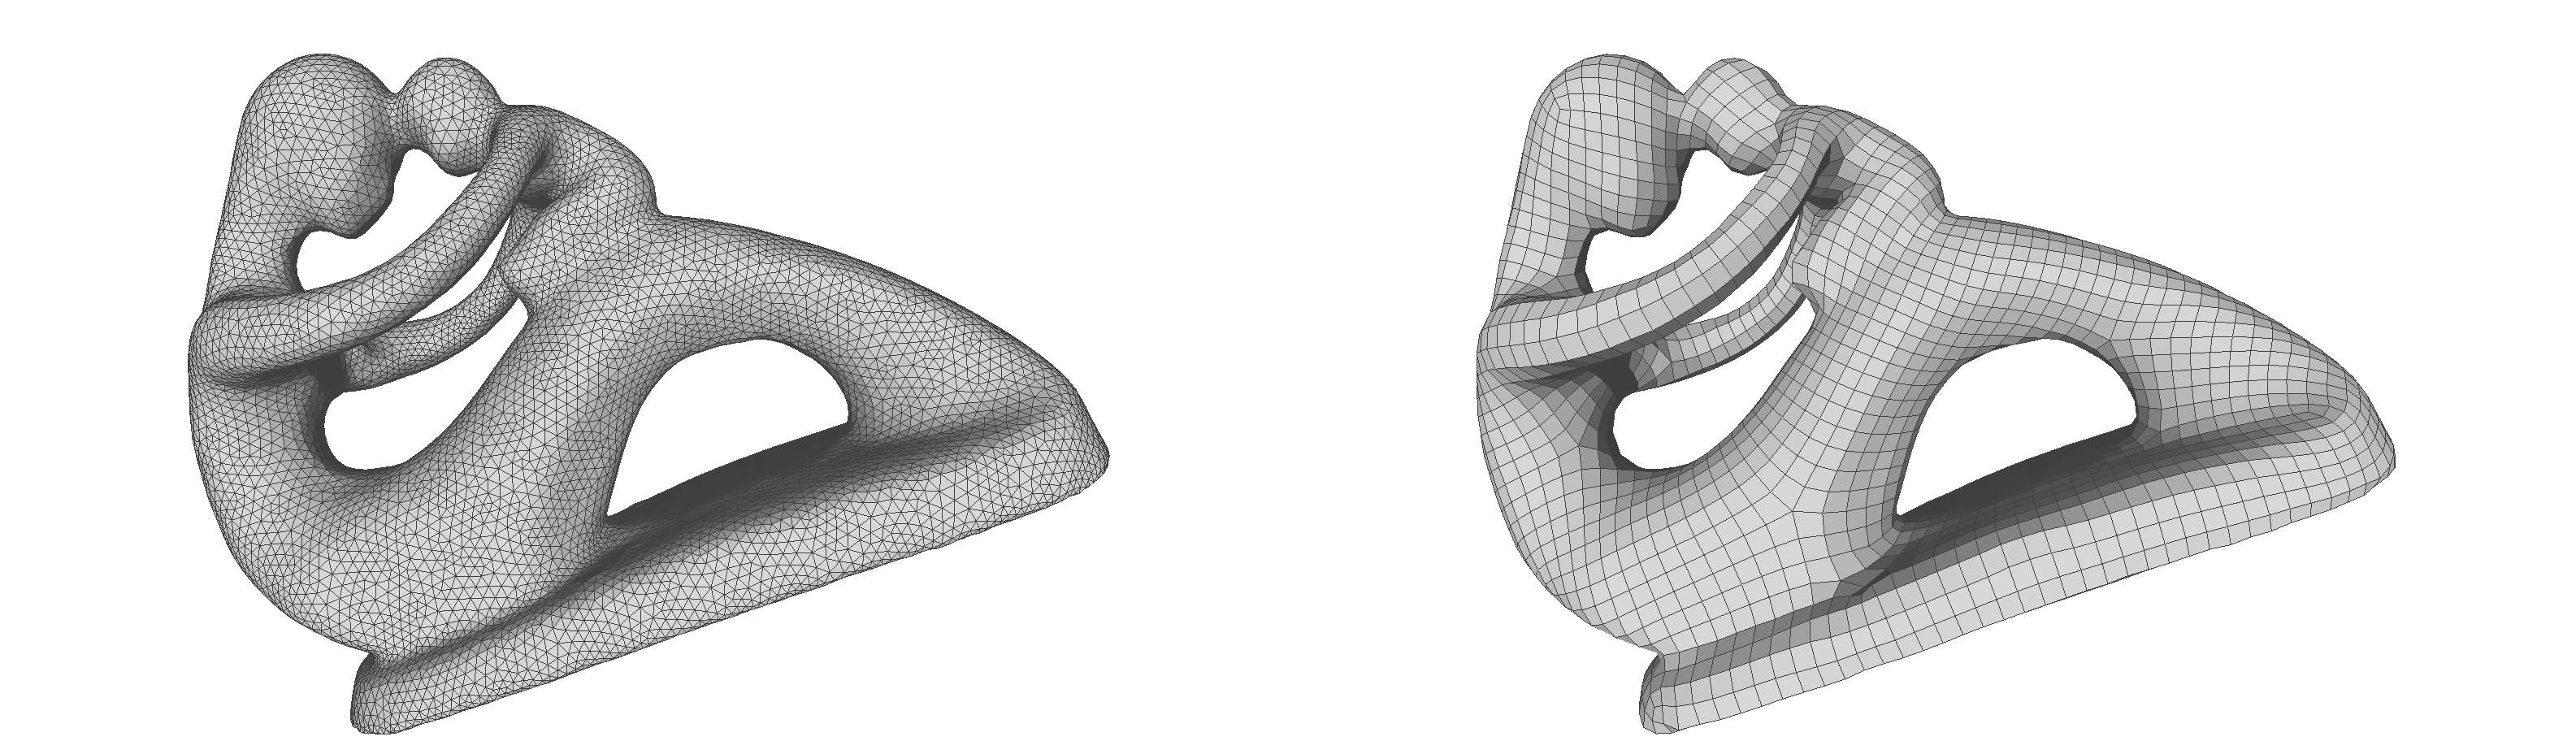
\includegraphics[width=15cm]{figures/tri_mesh_vs_quad_mesh.png}
\caption[Triangular mesh vs. Quad mesh]{A triangle-mesh (left) vs. a corresponding quad-mesh (right)}
\label{fig:tri_mesh_vs_quad_mesh}
\end{figure}

\subsection{Triangle Soup}
A \emph{triangle soup} is a formalization framework for describing a mapping of 2D manifold embedded in 3D onto the 2D Euclidean plane. In this formalization, every edge in the original mesh is treated as a cut seam, and therefore the input triangle-mesh is separated into individual triangles which are mapped onto the 2D domain.

\noindent Given that the input triangle-mesh is manifested as a tuple $M = (F,E,V)$, where $F$ is the set of facets, $E$ is the set of edges, and $V$ is the set of vertices, its triangle soup is given by $M_s = (F_s,E_s,V_s)$, where $\abs{F_s} = \abs{F}$, $\abs{E_s} = 2\abs{E} - \abs{E_{\partial M}}$, $\abs{V_s} = \sum_{v \in V} \mathrm{deg}(v) \cdot\abs{V}$, and $E_{\partial M}$ is the set of edges on the boundary of $M$ (if exists). Given a vertex $v_i$ of valence $k$ on $M$, and the triangle-fan adjacent to it (which constitutes a surface patch), we make the following notations:

\paragraph{Twin Edges} are two edges $e_i^k$ and $e_j^k$ on $M_s$ which corresponds to the same original edge $e_k$ on $M$.

\paragraph{Twin Vertices} are any two vertices $v_i^k$ and $v_j^k$ on $M_s$ which corresponds to the same original vertex $v_k$ on $M$.

\noindent Figure \ref{fig:triangle_soup} illustrates a surface patch which is mapped into the 2D domain as a triangle soup.

\begin{figure}[ht]
\centering
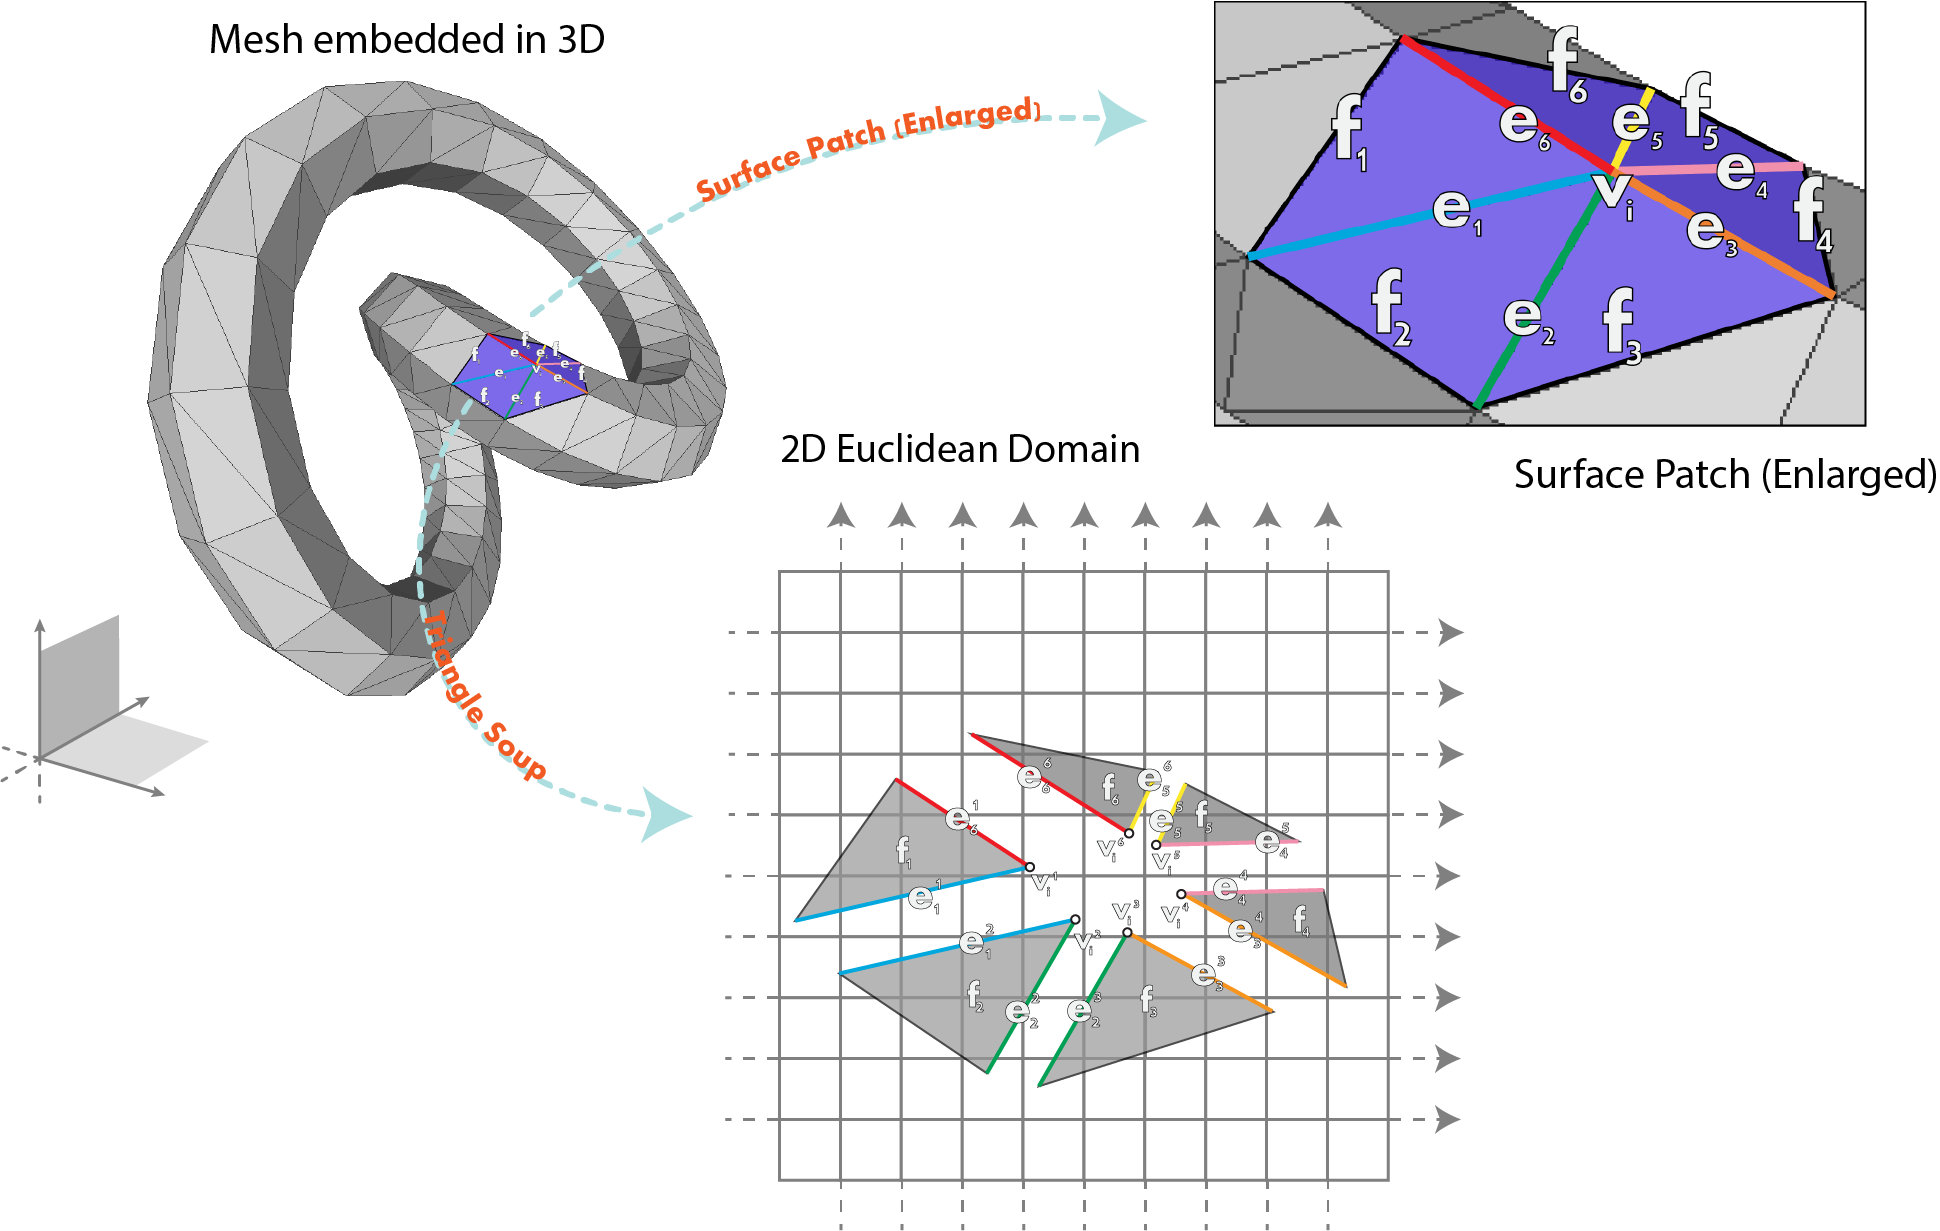
\includegraphics[width=16cm]{figures/triangle_soup.png}
\caption[Triangle Soup]{The purple surface patch, represented by the triangle-fan around vertex $v_i$, is mapped onto the 2D Euclidean domain as a triangle soup. Twin edges are highlighted by the same color on the 2D domain, and twin vertices are emphasized using a black stroked circle.}
\label{fig:triangle_soup}
\end{figure}

\subsection{Quad Meshes}
There are generally four types of quad meshes:

\begin{enumerate}
\item \textbf{Regular Quad Meshes} are quad meshes of which all their vertices are regular (valence 4). These type or meshes are relevant for disk or torodial (torus) topologies, and therefore, are limited in use.
\item \textbf{Semi-Regular Quad Meshes} are quad meshes which are made of 2D rectangular patches tessellated with quads, which are stitched together on the mesh's surface. This kind of meshes are highly useful due to their mostly regular nature (except for the possibly irregular vertices at the stitching points), but are also very hard to generate by remeshing methods.
\item \textbf{Valence Semi-Regular Quad Meshes} are quad meshes of which most of their vertices are of valence 4, but cannot be patched by stitching 2D patches. That is, a semi-regular quad mesh is also a valence semi-regular quad mesh, but not vice versa. These are the type of meshes which are usually produced by quad remeshing algorithms.
\item \textbf{Unstructured Quad Meshes} are quad meshes of which most of their vertices are irregular.
\end{enumerate}

\subsubsection{Irregular Vertices}
Irregular vertices are vertices of which their valence is different than 4. In other words, their immediate mesh neighbourhood do not resemble a 2D Cartesian grid. Quad remeshing techniques, on which we elaborate in the following chapters, produce valence semi-regular quad meshes which embed irregular vertices of valence 3 and 5 in order to compensate for Gaussian curvature. Figures \ref{fig:valence_3} and \ref{fig:valence_5} visualize the two types of irregular vertices.

\begin{figure}[ht]
\centering
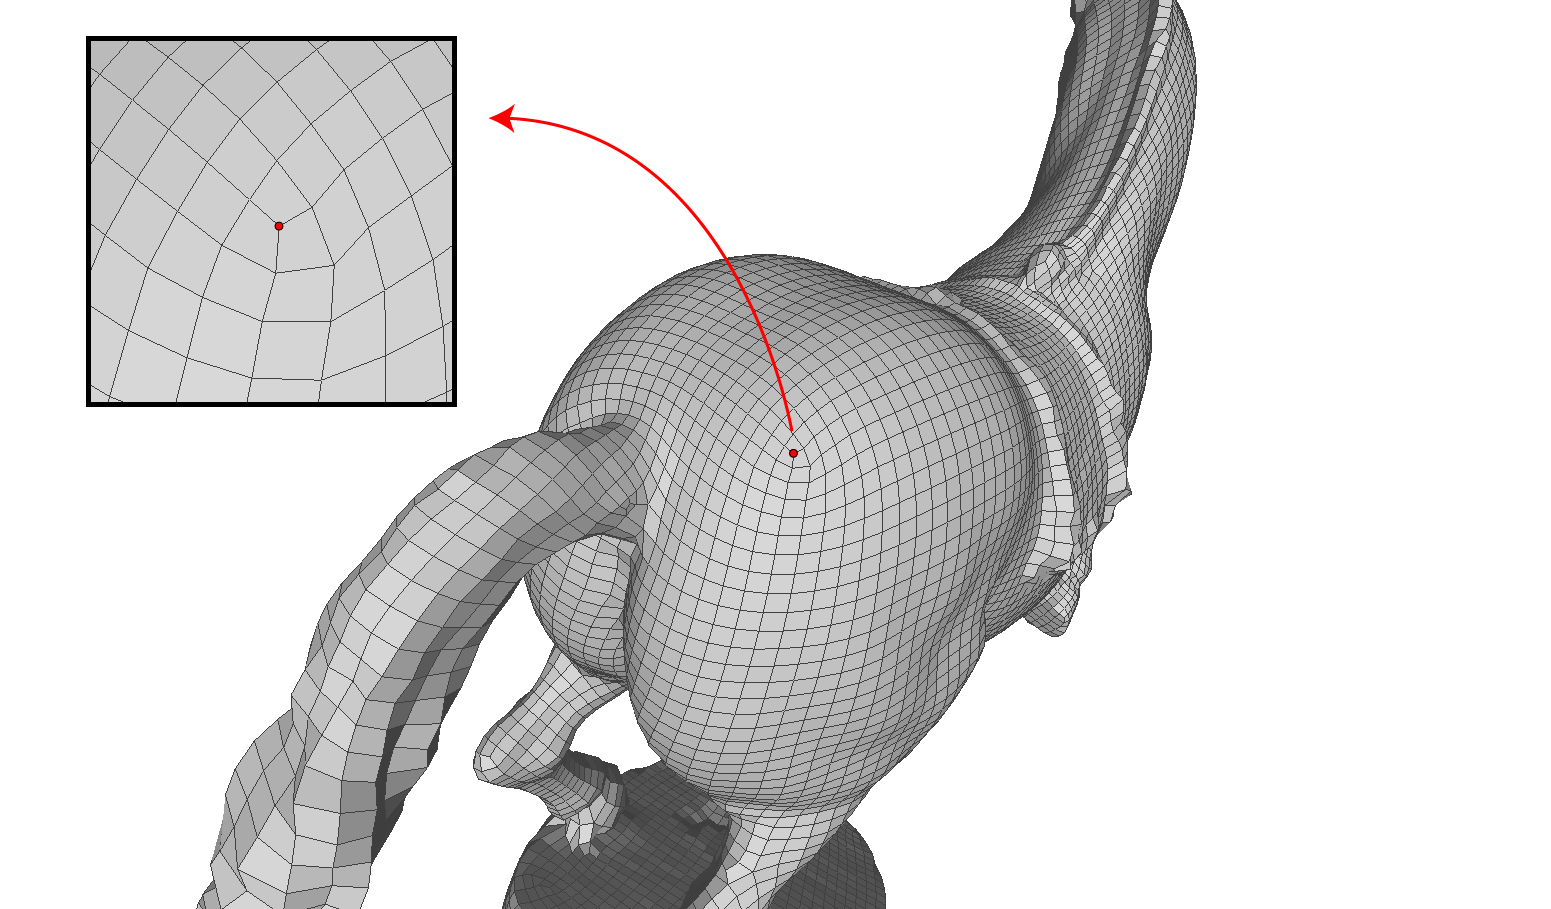
\includegraphics[width=13cm]{figures/valence_3.png}
\caption[Irregular vertex of valence 3]{The red dot indicates a vertex of valence 3 on the quadrangulated Rampant model}
\label{fig:valence_3}
\end{figure}

\begin{figure}[ht]
\centering
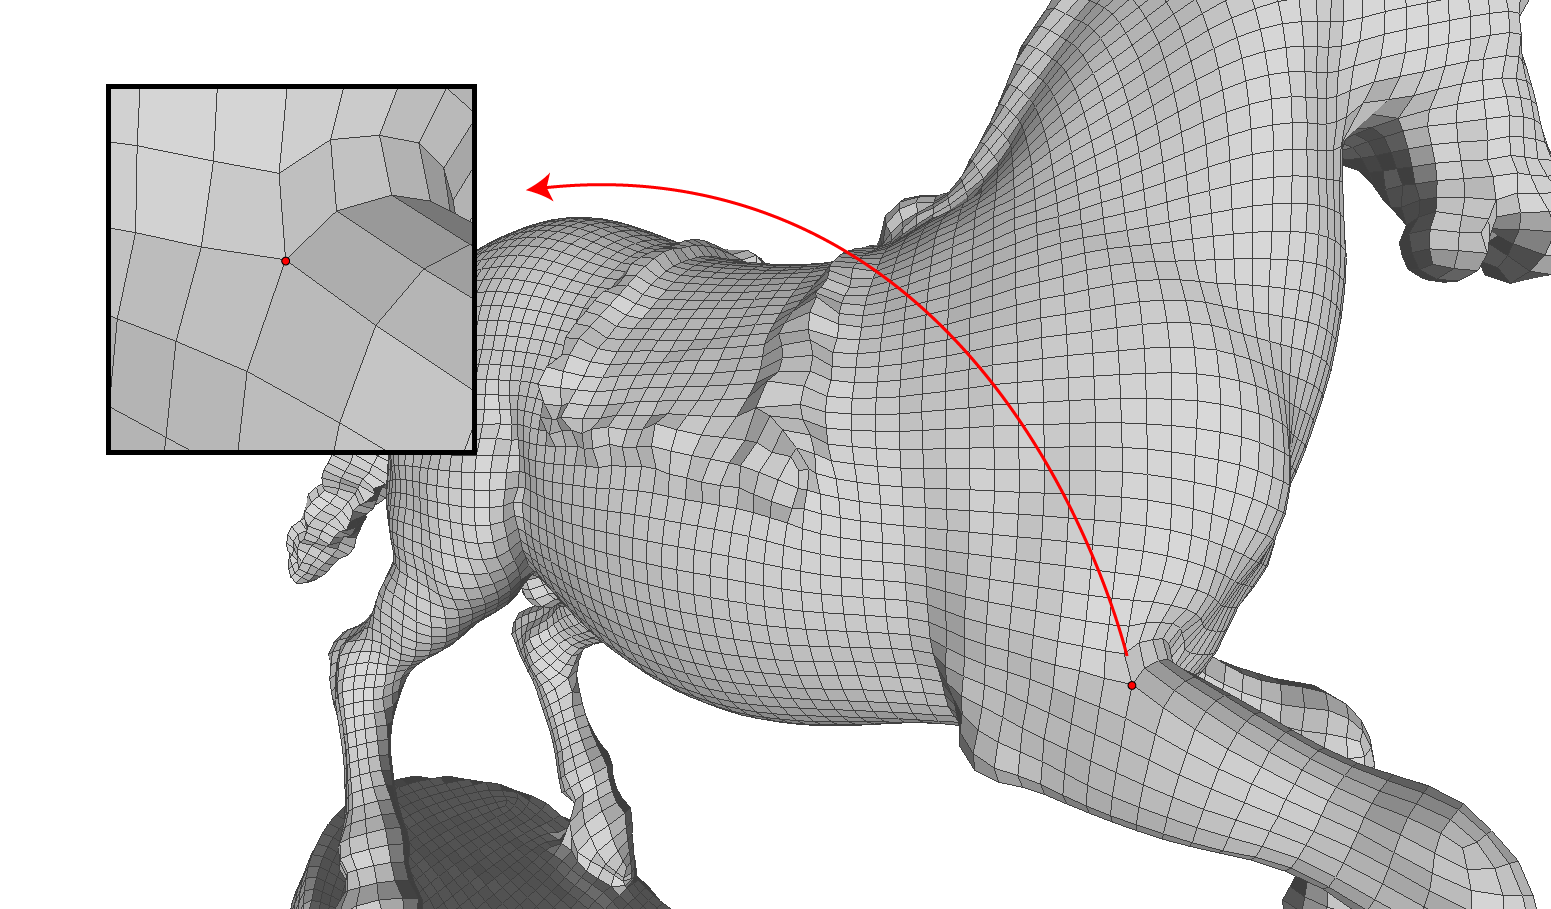
\includegraphics[width=13cm]{figures/valence_5.png}
\caption[Irregular vertex of valence 5]{The red dot indicates a vertex of valence 5 on the quadrangulated Rampant model}
\label{fig:valence_5}
\end{figure}

\subsubsection{Quad Mesh Quality}
Mesh models usually originates as unstructured triangle-meshes, and therefore, have to be converted into a semi-regular quad-meshes if the geometry-processing pipeline of a certain scenario requires it. In order to be able to compare between different conversion techniques, we have to define the quality measures, which are partially subjective, for a "good" quad-mesh.

\paragraph{Individual Quads Quality} If anisotropic quads are allowed or required, each quad should be close to
a 2D rectangle. Otherwise, it should be close to a 2D square. Specifically, it means that the the four vertices that make up the quads should be co-planar, opposite edges should have equal length and the four angles made up by consecutive edges should be close to $90^\circ$.

\paragraph{Curvature Alignment} Mesh edges should be oriented along curvature lines, except for points at flat areas where the curvature is zero.

\paragraph{Feature Alignment} Sharp geometric features of the mesh's surface should be traced by sequential mesh edges to get a quad mesh the approximates the original surface as good as possible.

\paragraph{Singular Points} The number of singular vertices, which are characterized by having valence an irregular valence (for example, 3 or 5), should be as small as possible, and their placement should be chosen or determined (automatically) such that the three former quality measures are maximized. Alternatively, their placement can be chosen to fit subjective artistic desires (for example, 3D character modeling).

\subsubsection{Applications}
Since points on smooth manifolds are characterized by two principal curvature directions (except for points on flat regions), quad-meshes are their natural approximators, since most vertices on a semi-regular quad-mesh are regular vertices of valence 4, of which their anti-symmetric edge pairs can be aligned with the principal curvature directions. This makes quad-meshes the desired approximations and representations of geometry in many types of applications.

\paragraph{3D Shape Modeling} In many cases, artists who design 3D models for entertainment and engineering purposes (video-games, animations, CAD, etc.) prefer to work in a quad-mesh settings, since their regular properties make it more intuitive to adapt their design to the geometric feature lines of their objects, which also provide better results under shape deformation.

\paragraph{Texturing} Since semi-regular quad-meshes are made of stitched together 2D rectangular quad grids, it is trivial to apply a set of textures and displacement-maps onto the 3D mesh.

\paragraph{Finite Element Simulations} Quad-meshes are preferred over triangle-meshes in finite-element simulation, since their regular nature reduce the approximation error and the number of mesh elements.

\paragraph{Shape Compression} The regular nature of quad-meshes, and especially of semi-regular quad-meshes, makes it possible to treat them as geometric images, due to their regularity, and apply on them image processing techniques such as image compression algorithms.

\section{Numerical Optimization}
Numerical optimization is a mathematical tool which grants its user the ability to minimize (or maximize) quantitative metric which usually measures the performance of the system under study. The metric to be optimized is expressed using a scalar objective which is a function of one or more system parameters. An \emph{optimization problem} is a problem which is satisfied by finding a point in the problem's domain where the objective metric is minimized (or maximized) locally or globally. Since we usually cannot find an analytic expression for the solution of an optimization problem, we have to solve it by iterative progression towards the solution using local approximations of the objective function in hand. An algorithm which iteratively converges to the solution is called an \emph{optimization method}. Numerical optimization methods are fundamental tools in all fields of engineering and science.

\noindent An optimization problem which has no restrictions on its domain is called an \emph{unconstrained optimization problem}. If we require that the solution will be restricted to a certain region of the domain, the problem is then called a \emph{constrained optimization problem}. Methods for solving unconstrained optimization problems are divided into two main types:
\begin{itemize}
    \item Trust Region Methods
    \item Line Search Methods
\end{itemize}

The following subsection contains a quick review for the two most common line-search unconstrained optimization methods: \emph{Gradient Descent} and \emph{Newton's Method}, of which we specifically use in the context of this work. For more information about Numerical Optimization, please refer to \cite{Nocedal2006Numerical}.
\paragraph{Important Remark} Every optimization problem can be formulated both as a minimization problem (by minimizing the objective function) or as a maximization problem (by maximizing the negative objective function). In this text, we assume that all optimization problems are formulated as minimization problems.
\subsection{Quadratic Approximation}
Given a scalar function:
$$f:\mathbb{R}^2\rightarrow\mathbb{R}$$
We know by the multivariate Taylor's theorem that its quadratic approximation $q\left(x,y\right)$ at the point $\left(x_0,y_0\right)$ is given by:
\begin{equation}\label{quadratic_approx}
\begin{split}
f\left(x,y\right) \approx f\left(x_0,y_0\right) + f_x\left(x_0,y_0\right)\left(x - x_0\right) + f_y\left(x_0,y_0\right)\left(y - y_0\right) \\ + \frac{1}{2}f_{xx}\left(x_0,y_0\right)\left(x - x_0\right)^2 + \frac{1}{2}f_{xy}\left(x_0,y_0\right)\left(x - x_0\right)\left(y - y_0\right) \\ +  \frac{1}{2}f_{yx}\left(x_0,y_0\right)\left(x - x_0\right)\left(y - y_0\right) + \frac{1}{2}f_{yy}\left(x_0,y_0\right)\left(y - y_0\right)^2
\end{split}
\end{equation}
By factorizing (\ref{quadratic_approx}) we get the following:
\begin{equation}\label{factorized_quadratic_approx}
\begin{split}
f\left(x,y\right) \approx f\left(x_0,y_0\right) + f_x\left(x_0,y_0\right)\left(x - x_0\right) + f_y\left(x_0,y_0\right)\left(y - y_0\right) \\ + \frac{1}{2}\Big(\left(x - x_0\right)\big( f_{xx}\left(x_0,y_0\right) \left(x - x_0\right) + f_{xy}\left(x_0,y_0\right) \left(y - y_0\right) \big) \\ + \big( f_{yx}\left(x_0,y_0\right) \left(x - x_0\right) + f_{yy}\left(x_0,y_0\right) \left(y - y_0\right) \big)\left(y - y_0\right)\Big)
\end{split}
\end{equation}
By denoting:
$$
p = 
\begin{pmatrix}
x\\
y\\
\end{pmatrix},
p_0 = 
\begin{pmatrix}
x_0\\
y_0\\
\end{pmatrix},
\nabla f\left(x_0,y_0\right) = 
\begin{pmatrix}
f_x\left(x_0,y_0\right)\\
f_y\left(x_0,y_0\right)\\
\end{pmatrix},
\nabla^2 f\left(x_0,y_0\right) = 
\begin{pmatrix}
f_{xx}\left(x_0,y_0\right) & f_{xy}\left(x_0,y_0\right)\\
f_{yx}\left(x_0,y_0\right) & f_{yy}\left(x_0,y_0\right)
\end{pmatrix}
$$
We can rewrite (\ref{vectorized_quadratic_approx}) in a vectorized form by:
\begin{equation}\label{vectorized_quadratic_approx}
\begin{split}
f\left(p\right) \approx f\left(p_0\right) + \nabla f\left(p_0\right)^T\left(p-p_0\right) + \frac{1}{2}\left(p-p_0\right)^T\nabla^2 f\left(p_0\right)\left(p-p_0\right)
\end{split}
\end{equation}

\noindent The right side of (\ref{vectorized_quadratic_approx}) is called the \emph{quadratic approximation} of $f(p)$ at the point $p=(x_0, y_0)$, and is denoted by $Q(p)$.

\noindent The derivation above was done for the two-dimensional case, however, it is possible to generalize the derivation and show that the vectorized end result is the same for $f:\mathbb{R}^n\rightarrow\mathbb{R}$ with an arbitrary $n$.

\noindent The geometric interpretation of the quadratic approximation of a function at a point $p_0$ is a hyper-paraboloid that passes through $p_0$ which best approximates the function $f(p)$ around any small neighbourhood of $p_0$.

\begin{figure}[ht]
\centering
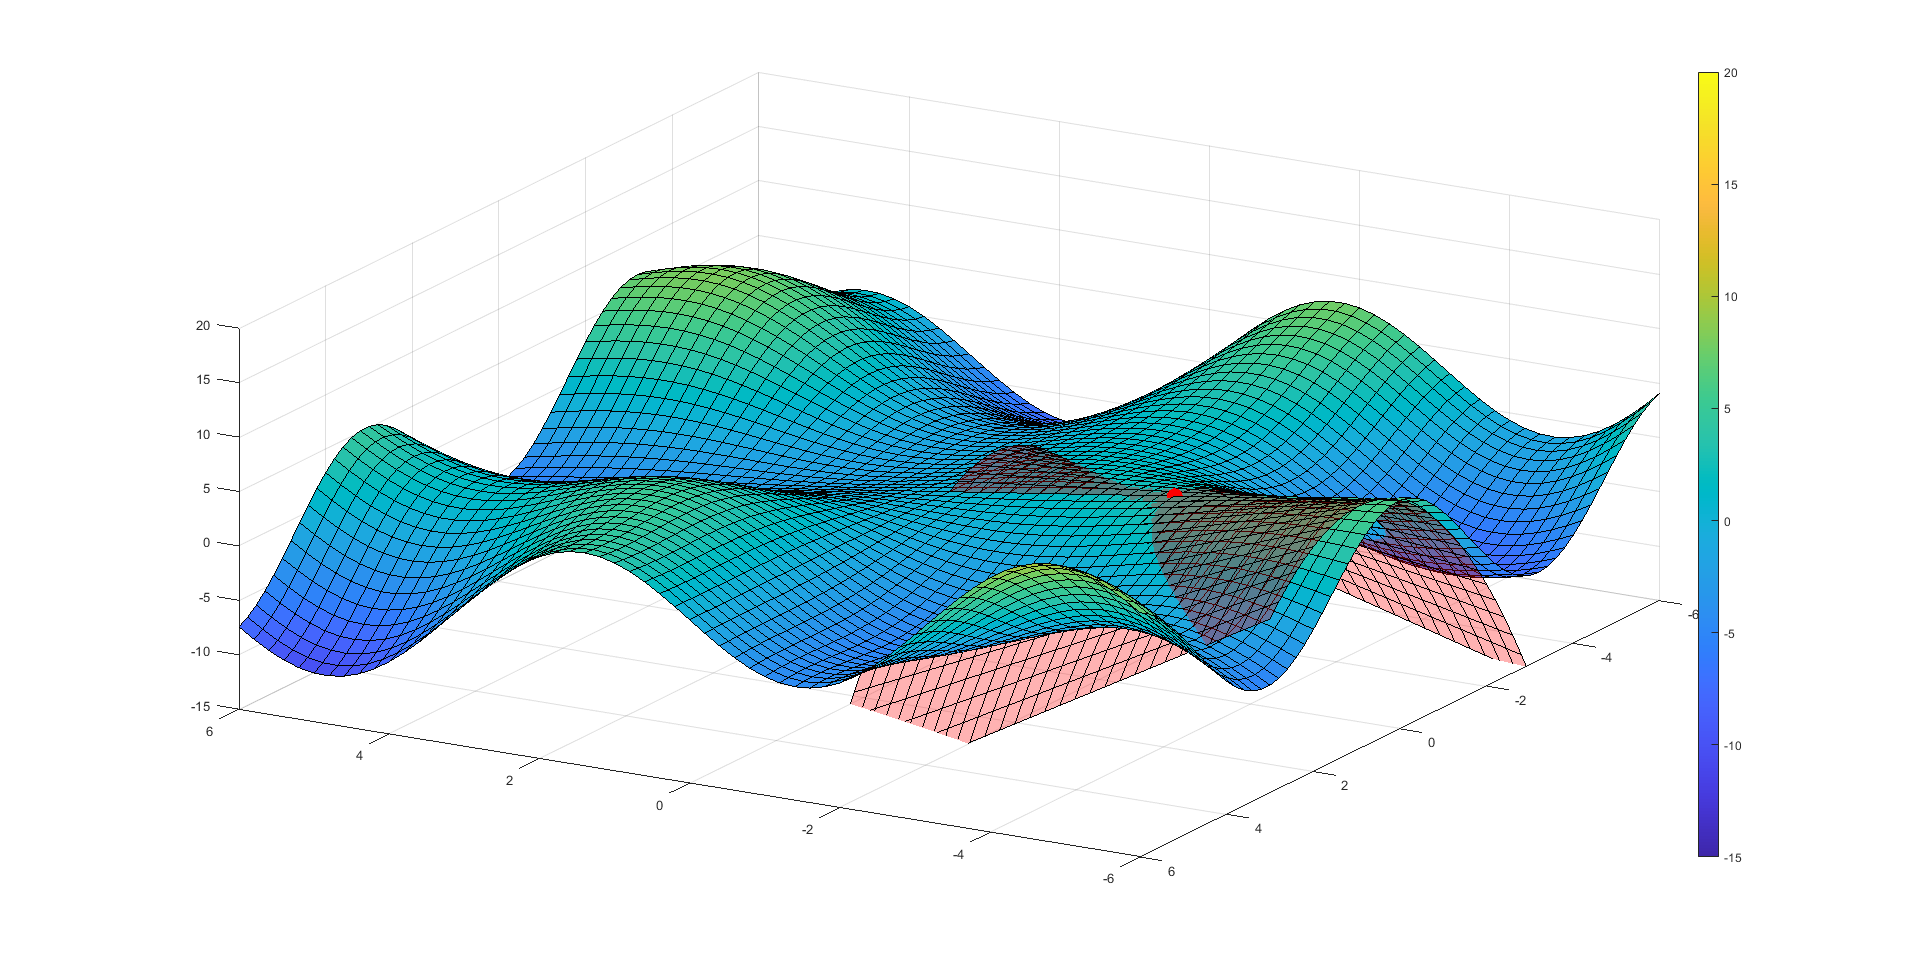
\includegraphics[width=13cm]{figures/quad_approx1}
\caption[Quadratic approximation example 1]{Example plot of the quadratic approximation (the red paraboloid) of the function $f\left(x_0, x_1\right) = x_2sin\left(x_1\right) - x_1cos\left(x_2\right)$ at the point $p_0 = \left(4.4, 0.4\right)$ (the red dot)}
\label{fig:quad_approx1}
\end{figure}

\begin{figure}[ht]
\centering
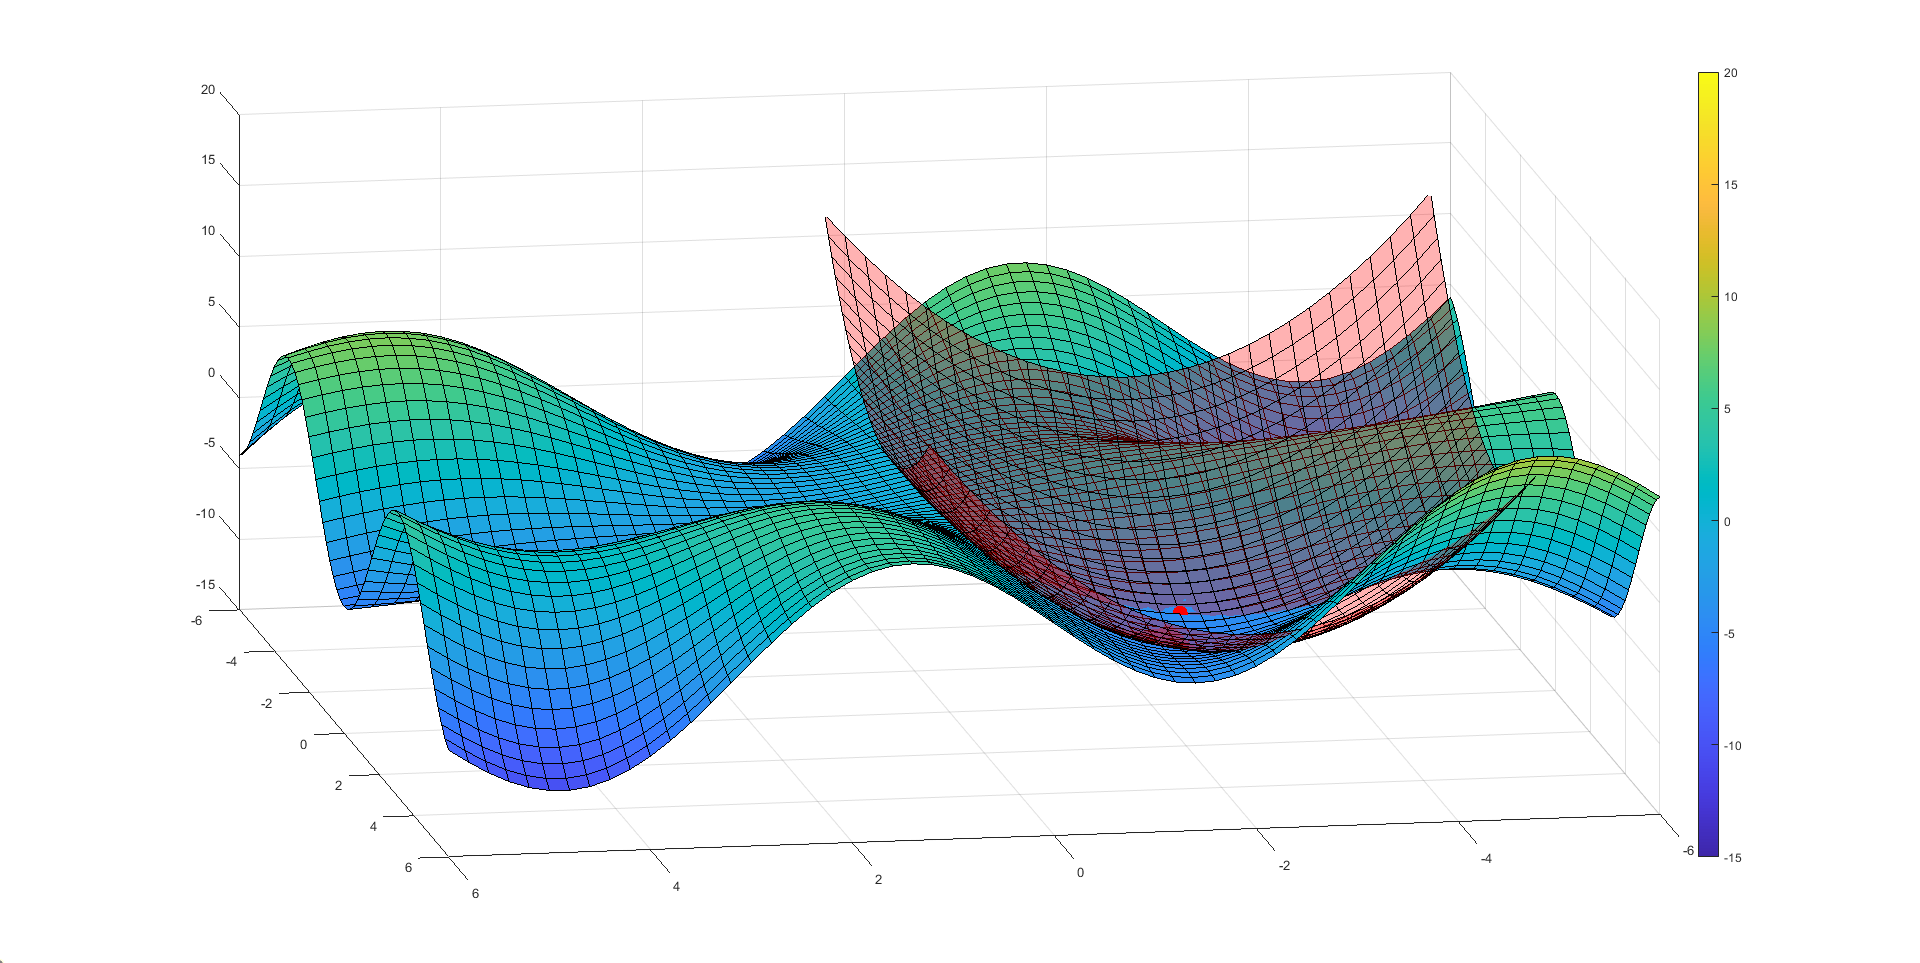
\includegraphics[width=13cm]{figures/quad_approx2}
\caption[Quadratic approximation example 2]{Another example plot of the quadratic approximation (the red paraboloid) of the function $f\left(x_0, x_1\right) = x_2sin\left(x_1\right) - x_1cos\left(x_2\right)$ at the point $p_0 = \left(-1.8, 2.8\right)$ (the red dot)}
\label{fig:quad_approx2}
\end{figure}

\subsection{Linear Approximation}
By omitting the quadratic form from equation (\ref{vectorized_quadratic_approx}) to we get:
\begin{equation}\label{vectorized_linear_approx}
\begin{split}
f\left(p\right) \approx f\left(p_0\right) + \nabla f\left(p_0\right)^T\left(p-p_0\right)
\end{split}
\end{equation}

\noindent The right side of (\ref{vectorized_linear_approx}) is called the \emph{linear approximation} of $f(p)$ at the point $p=(x_0, y_0)$, and is denoted by $L(p)$.

\noindent The geometric interpretation the linear approximation of a function at a point $p_0$ is a hyperplane that passes through $p_0$ which best approximates the function $f(p)$ around any small neighbourhood of $p_0$.

\begin{figure}[ht]
\centering
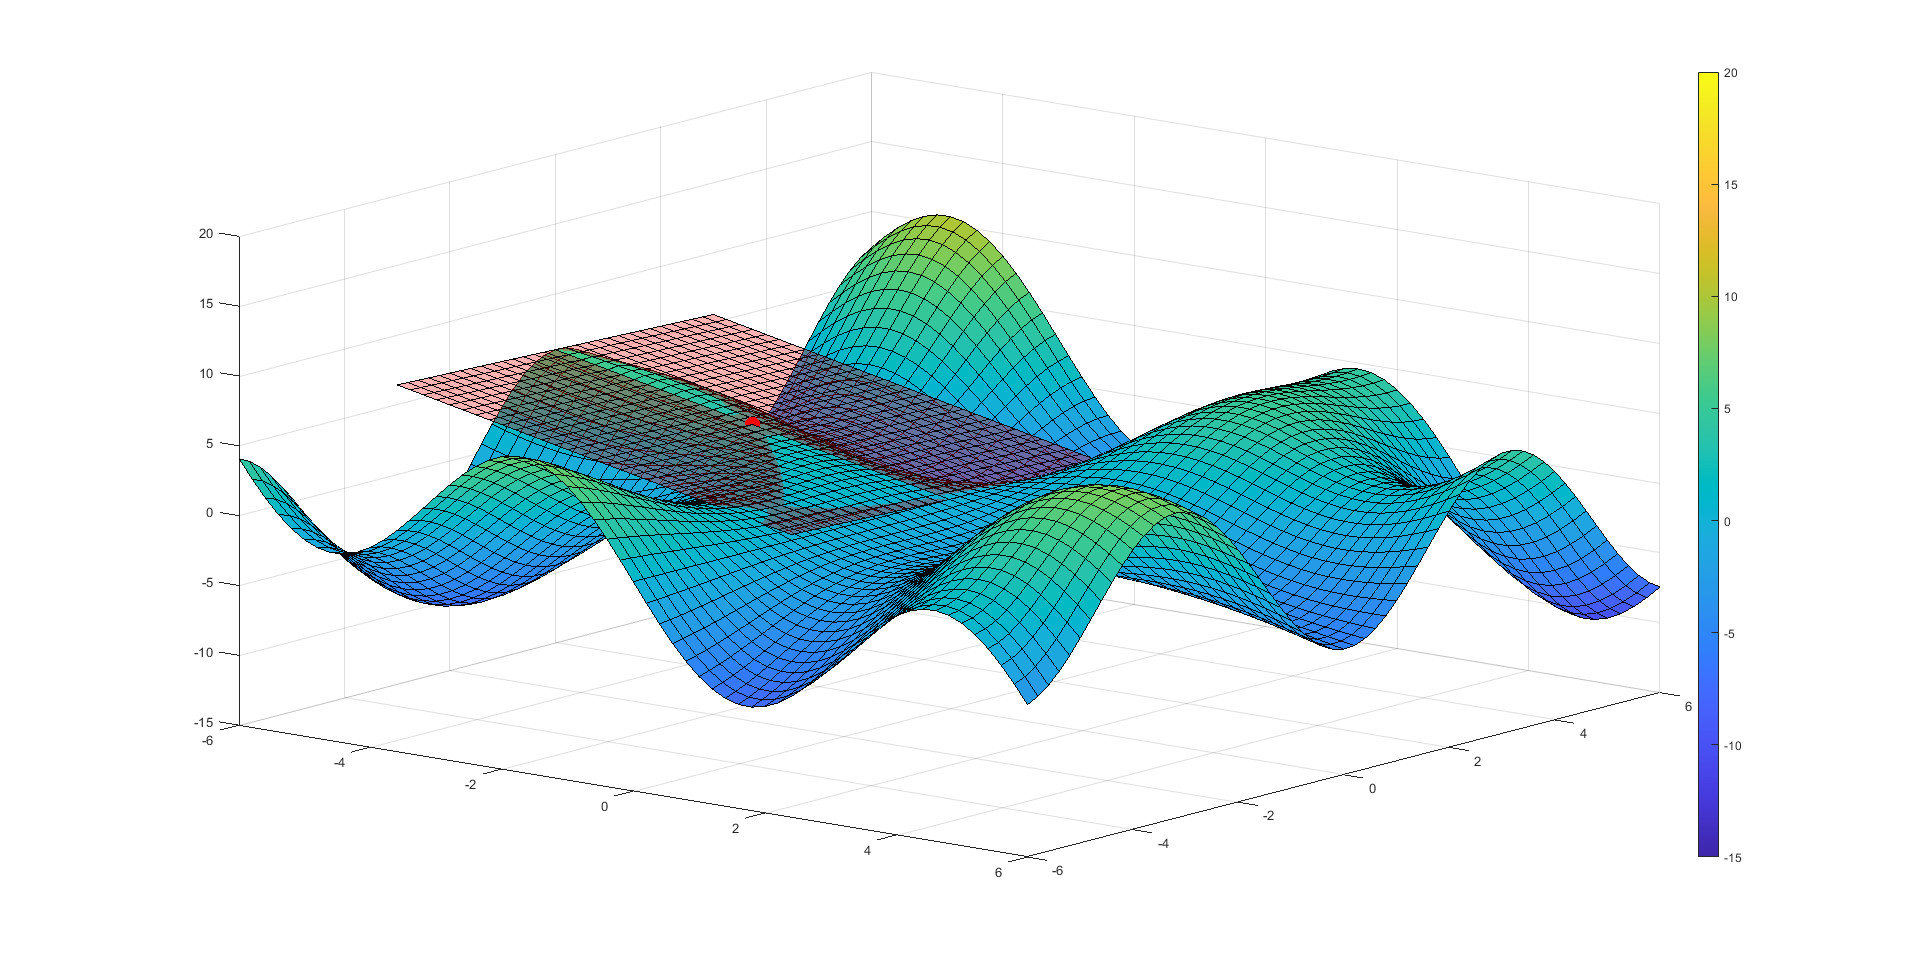
\includegraphics[width=13cm]{figures/linear_approx1}
\caption[Linear approximation example 1]{Example plot of the linear approximation (the red plane) of the function $f\left(x_0, x_1\right) = x_2sin\left(x_1\right) - x_1cos\left(x_2\right)$ at the point $p_0 = \left(0, -3\right)$ (the red dot)}
\label{fig:linear_approx1}
\end{figure}
\begin{figure}[ht]
\centering
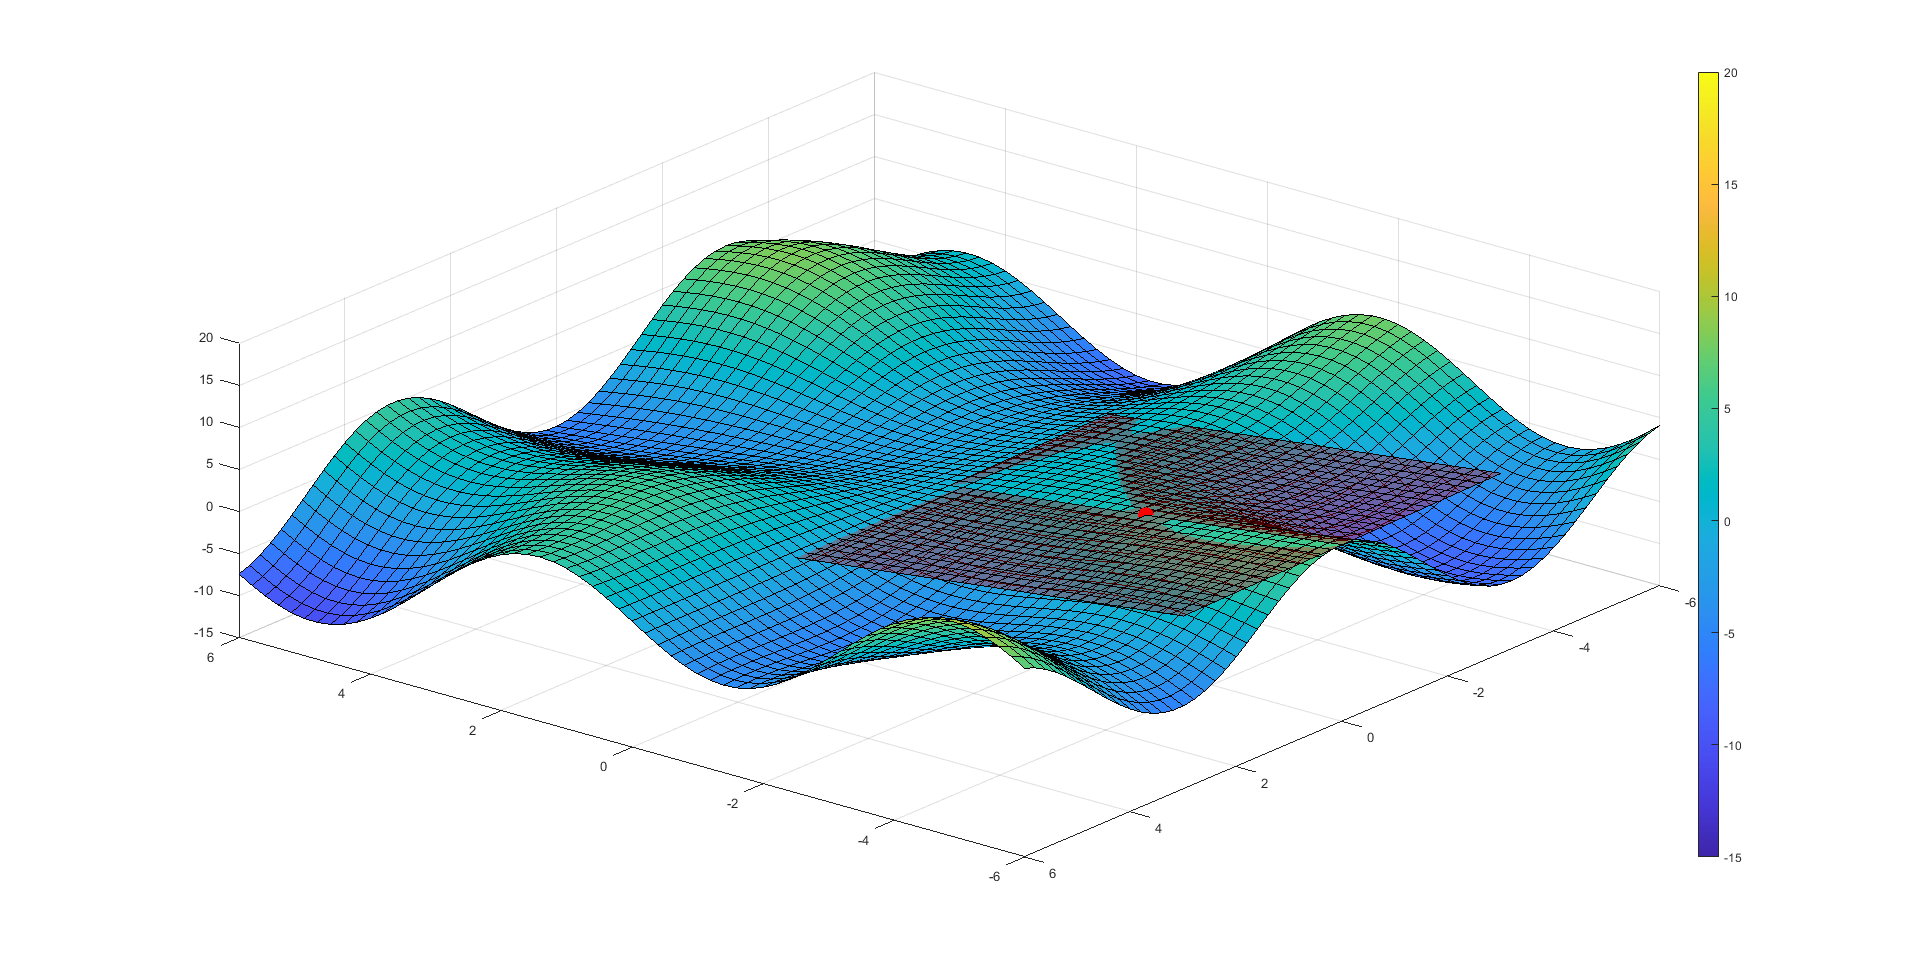
\includegraphics[width=13cm]{figures/linear_approx2}
\caption[Linear approximation example 2]{Plot from a different angle of the same linear approximation from figure \ref{fig:linear_approx1}}
\label{fig:linear_approx2}
\end{figure}

\subsection{Gradient Descent}
Gradient Descent is a first-order iterative line-search algorithm, of which at its $i$th iteration takes a single step in the direction of $-\nabla f\left(p_i\right)$ (the negative gradient direction, calculated at the point $p_i$). To see why, assume that we're given a function $f:\mathbb{R}^n\rightarrow\mathbb{R}$ and a point $p_i$ in its domain. We would like to find a new point $p_{i+1}$, which together with $p_i$, will provide the direction of steepest descent on the linear approximation of $f(p)$ at the point $p_i$. The linear approximation of $f$ at $p_i$ is given by:
\begin{equation}
\label{vectorized_quadratic_approx_p}
\begin{split}
L\left(p\right) = f\left(p_i\right) + \nabla f\left(p_i\right)^T\left(p-p_i\right)
\end{split}
\end{equation}
Let's denote $d_i = p-p_i$. By the definition of the inner-product, if we take $d_i = -\widehat{\nabla f}\left(p_i\right)$ as unit-vector that represent the direction of progression, we will achieve maximal decrease in $L\left(p\right)$ out of all possible unit-vector directions. This mean that we would like to choose $p_{i+1}$ somewhere along the ray emitted from $p_i$ in direction $-\widehat{\nabla f}\left(p_i\right)$. That is, we're looking for a step-size $\alpha_i>0$ such that by  taking $p_{i+1}=p_i - \alpha \widehat{\nabla f}\left(p_i\right)$ we will achieve a sufficient decrease in $f\left(p_{i+1}\right)$. That quest for finding the correct step-size along a ray is called \emph{Line Search}.
Pseudo-code for the vanilla versions of the Line-Search and Gradient Descent algorithms are given in Algorithms \ref{alg:line_search_algorithm} and \ref{alg:gradient_descent_algorithm}, respectively. The Gradient Descent algorithm converges linearly to a local minimum point of $f$. However, there is always a risk that the process get to a sudden halt at a saddle point, where the gradient is zero. For further reading, please refer to \cite{Nocedal2006Numerical}.
\begin{algorithm}[ht]
  \caption{Line Search Algorithm}
  \label{alg:line_search_algorithm}
  \begin{algorithmic}[1]
    \Function {LineSearch}{$f$, $p$, $d$, $\alpha_0$}
    \State $\emph{sufficient} \leftarrow false$
    \State $\alpha \leftarrow \alpha_0$
    \State $v \leftarrow f\left(p\right)$
    \Repeat
        \State $p_{next} \leftarrow p + \alpha d$
        \State $v_{next} \leftarrow f\left(p_{next}\right)$
        \State $\alpha \leftarrow \frac{\alpha}{2}$
        \If {$v_{next} < v$}
            \State $\emph{sufficient} \leftarrow true$
        \EndIf
    \Until{$\emph{sufficient}$}
    \State \Return $p_{next}$
    \EndFunction
  \end{algorithmic}
\end{algorithm}
\begin{algorithm}[ht]
  \caption{Gradient Descent Algorithm}
  \label{alg:gradient_descent_algorithm}
  \begin{algorithmic}[1]
    \Function {GradientDescent}{$f$, $\nabla f$, $p_0$, $\alpha$, $\epsilon$}
      \State $i \leftarrow 0$
      \While{$ \norm{ \nable f \left( p_i \right) }_2 > \epsilon$}
        \State $d_i \leftarrow -\nabla f \left(p_i\right)$
        \State $p_{i+1} \leftarrow \Call{LineSearch}{f, p_i, d_i, \alpha}$
        \State $i \leftarrow i + 1$
      \EndWhile
      \State \Return $p_i$
    \EndFunction
  \end{algorithmic}
\end{algorithm}

\subsection{Newton's Method}
Newton's Method is a second-order iterative line-search algorithm. In contrast to the Gradient Descent algorithm, which is based on the linear (first order) approximation of $f$ at point $p_i$, Newton's Method is based on the quadratic (second order) approximation of $f$ at point $p_i$. If the quadratic approximation of $f$ at a given point is a convex hyper-paraboloid, it has a minimum point $q_{min}$. Since a quadratic approximation of a function $f$, at point $p_i$, gives a good approximation of $f$ at a small neighbourhood of $p_i$, it make sense that by stepping along the ray (in $f$'s domain space) emitted from $p_i$ in direction $d_i = q_{min} - p_i$ will yield a new point $p_{i+1}$ which provide sufficient decrease in $f$.
In order to determine $d_i$, we first have to find the minimum point of the quadratic approximation of $f$ at point $p_i$. By equation (\ref{vectorized_quadratic_approx}), we know that the quadratic approximation of $f\left(p_i\right)$ is given by:
\begin{equation}\label{vectorized_quadratic_approx_p}
\begin{split}
Q\left(p\right) = f\left(p_i\right) + \nabla f\left(p_i\right)^T\left(p-p_i\right) + \frac{1}{2}\left(p-p_i\right)^T\nabla^2 f\left(p_i\right)\left(p-p_i\right)
\end{split}
\end{equation}
We first note that:
\begin{equation}\label{d_i_p_i_p}
\begin{split}
d_i = p - p_i \implies p = p_i + d_i
\end{split}
\end{equation}
Plugging \ref{d_i_p_i_p} into equation \ref{vectorized_quadratic_approx_p}, we get:
\begin{equation}\label{vectorized_quadratic_approx_p_i_d_i}
\begin{split}
Q\left(p_i + d_i\right) = f\left(p_i\right) + \nabla f\left(p_i\right)^Td_i + \frac{1}{2}d_i^T\nabla^2 f\left(p_i\right)d_i
\end{split}
\end{equation}
By differentiating equation \ref{vectorized_quadratic_approx_p_i_d_i} by $d_i$, we get that:
\begin{equation}\label{newton_equation}
\begin{split}
\nabla Q\left(p_i + d_i\right) = \nabla f\left(p_i\right) + \nabla^2 f\left(p_i\right)d_i
\end{split}
\end{equation}
By setting $\nabla Q\left(p_i + d_i\right) = 0$ (in order to find the minimum point) and plugging back into equation \ref{newton_equation}, we get that:
\begin{equation}\label{newton_equation}
\begin{split}
d_i = -\nabla^2 f\left(p_i\right)^{-1} \nabla f\left(p_i\right)
\end{split}
\end{equation}
Equation \ref{newton_equation} gives us an explicit expression for the vector $d_i$, which takes us from the point $p_i$, to the minimum point of the paraboloid which forms the quadratic approximation of $f$ at point $p_i$. By expanding this idea further, we can normalize $d_i$ to be a unit vector, and use it as a direction of search for a line-search method.
\paragraph{Important Remark} In order for the quadratic approximation of $f$ in point $p_i$ to have minimum point, its Hessian $\nabla^2 f\left(p_i\right)$ has to be positive semi-definite matrix, which means that it has to have non-zero singular values. The geometric meaning of that, is that the hyper-paraboloid represented by the quadratic approximation of $f$ in $p_i$ should be convex. In case it doesn't, we can use the \emph{SVD decomposition} to reassemble $\nabla^2 f\left(p_i\right)$ into its closest approximation which doesn't have any non-zero singular value. For more information about SVD decomposition, please see \cite{strang2006linear}.

Pseudo-code for a vanilla version of the Newton's Method algorithm is given in Algorithm \ref{alg:newton_method_algorithm}. The Newton's Method algorithm converges quadratically to a local minimum point of $f$, given certain conditions are met. For further reading, please refer to \cite{Nocedal2006Numerical}.
\begin{algorithm}[ht]
  \caption{Newton's Method Algorithm}
  \label{alg:newton_method_algorithm}
  \begin{algorithmic}[1]
    \Function {NewtonMethod}{$f$, $\nabla f$, $p_0$, $\alpha$, $\epsilon$}
      \State $i \leftarrow 0$
      \While{$\norm{\nable f\left(p_i\right)}_2 > \epsilon$}
        \State $d_i \leftarrow -\nabla^2 f\left(p_i\right)^{-1} \nabla f\left(p_i\right)$
        \State $p_{i+1} \leftarrow \Call{LineSearch}{f, p_i, d_i, \alpha}$
        \State $i \leftarrow i + 1$
      \EndWhile
      \State \Return $p_i$
    \EndFunction
  \end{algorithmic}
\end{algorithm}